\subsection{Implementation}

\subsubsection{Auto-complete}

	\paragraph{Introduction} \hspace{1mm}\\
	The customer wanted the application to auto-complete species names as they were typed in.
	That means when someone wants to enter an observation for a species and starts typing in species names, the application will suggest names based on what the user has typed in so far.
	This will help speed up the use of the application and also help with reducing typographical errors (typoes).

	Artsdatabanken provided us with an XML API on our customer meeting on September 13th so we can get the list of names for all the species to be used with auto-complete.
	We needed to download XML documents separately for each species group containing loads of information (~40 MB for butterflies).
	Amongst these documents two were massive, with one containing over half a million lines of xml data.
	Three were quite big, another three fairly small with the rest almost empty. With a total of 30 categories at the time, several of which will most likely not be used.

	The API could not be used as is because the application needs to use this feature while offline. Because of this, these generated XML files would have to be downloaded for use offline.

	\paragraph{Processing}  \hspace{1mm}\\
	The files collected from the Artsdatabanken were quite extensive, containing a lot more information than needed, and in their raw form would take up unreasonably large space on the phones memory.
	Because of this we had to parse the xml files into other a more usable format, at first we created a new xml file with just the information needed.
	This was slightly tweaked by making json files instead.

	All the data was downloaded from
\newline"http://webtjenester.artsdatabanken.no/Artsnavnebase.asmx/Artstre? \newline LatinskNavnID=\textless species id\textgreater\&Dybde=-1".
	Where \textless species id\textgreater ranges from 75 to 105. "Dybde" or depth in english, signifies that the fetched xml file should contain all species in the entire subtree.
	The API interface used generates a species list organized in a tree structure, based on subgroups of species with a lot of additional information.

	The only information we needed to use were the norwegian and scientific names, therefore we created an xml parser using a php script that generated an XSLT (Extensible Stylesheet Language Transformation\cite{w3:xslt}) of the xml file to be transformed into whatever format we liked.
	Because many names are the same in both Norwegian Bokm�l and Norwegian Nynorsk and for other reasons there were duplicates, the file was sorted, duplicates removed and json code inserted to make it ready for use.

	\paragraph{Processing impact} \hspace{1mm}\\
	The API used to generate this data seems to be very heavy on the server, only to generate a file of a few megabytes required up to 20 seconds.
	And with the largest file passing 40 megabytes and minutes to generate this functionality does not at this point seem like something you want the user to do regularly, or even at all.
	For the time being we will include the parsed files with the aplication and update the data by rolling out a new version of the application.

	Even if this only required to download the 80 megabytes and consume a lot of resources locally on the phone for some minutes, the perceived impact on the Artsdatabanken server from our view seemed significant. While not entirely sure, it is highly likely that it was our constant downloading of these complete XML files that might have caused the crash ,for a little bit of time, on the NTNU server hosting the API, see figure ~\ref{fig:artsdatabanken_api}.

	\begin{figure}[htb]
	\centering
	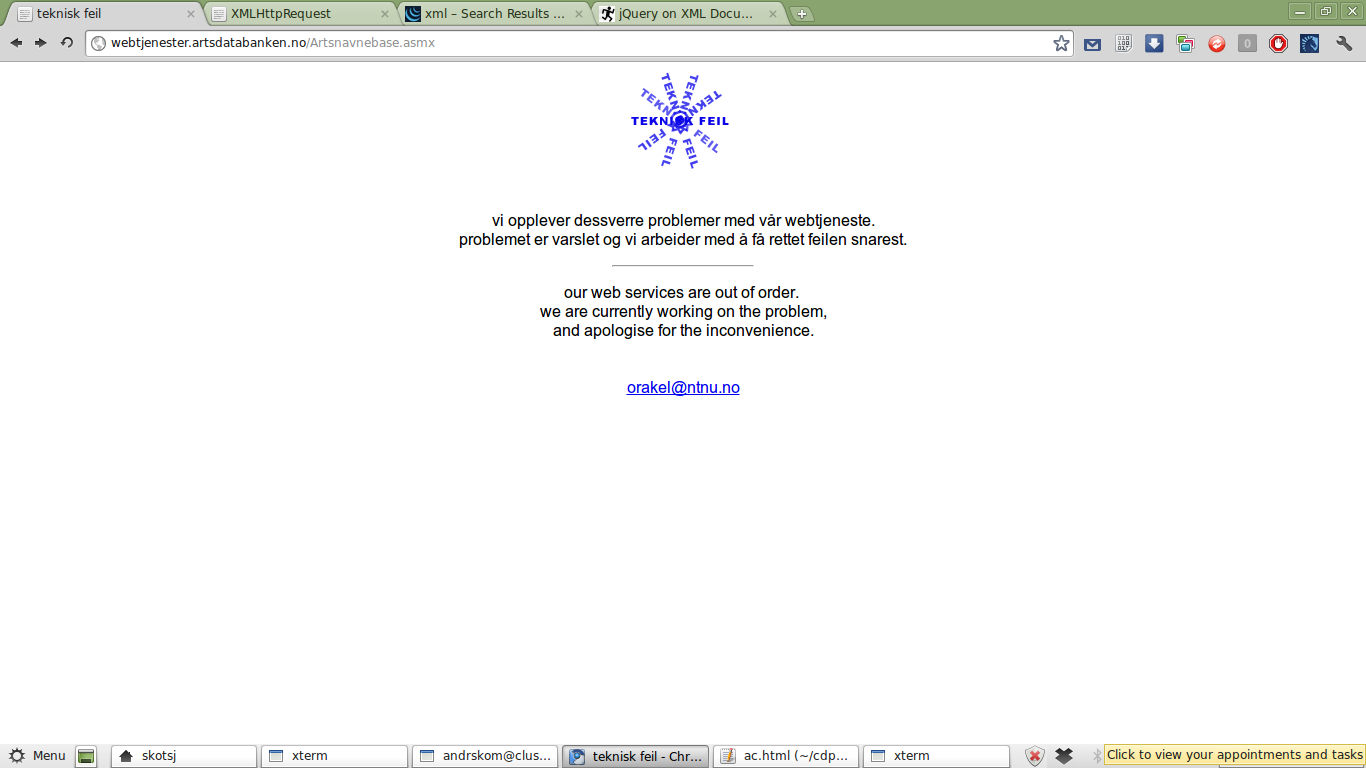
\includegraphics[width=1\textwidth]{implementation/preparation/ntnu_server_artsdatabanken.png}
	\caption{Artsdatabanken after downloading some of the xml}
	\label{fig:artsdatabanken_api}
	\end{figure}

	\paragraph{Implementation} \hspace{1mm}\\
		To download, and transform the data into a suitable format we used the
		following algorithm:

		\begin{enumerate}
			\item Download XML data from Artsdatabanken, one file per species category
			\item Pull relevant names from each XML file and store in flat text files (comma separated)
			\item Sort flat files
			\item Remove duplicate entries
			\item Enclose list structures in a JavaScript functions (var
			funcname = function() \{return [ ... list items ... ]; \}
		\end{enumerate}

		Step 5 is included to follow the JSONP standard, i.e. data
		that can be included in a normal script tag.

		Initially we planned on doing all the processing using PHP. This worked
		well for smaller data sets but we encountered problems as the file
		sizes grew. While trying to download big files PHP timed out due to the
		long waiting time (slow server response). This could probably be
		amended by changing some configurations, but that would not give a
		portable solution. Instead we decided to take advantage of the great
		linux terminal, bash.

		The final solution consists of a shell script, PHP, XSLT and a makefile
		to pull it all together.  Downloading, sorting, and removal of
		duplicate entries are done by a shell script (using wget, sort and
		uniq). An XSLT file defines how the XML files should be translated, and
		PHP drives the XSLT transformation.

		To update the auto-complete base, all we need to do is to run the
		following commands (download and parse XML, remove temporary files):
\begin{lstlisting}
make
make clean
\end{lstlisting}

